\chapter{Deutsch's Algorithm}

 In 1985, David Deutsch, a physicist at the University of Oxford, first discovered a problem that could be solved by a quantum computer faster than a classical computer. This is one of the simpler quantum algorithms in this section, which are admittedly more of intellectual curiosities than practical tools. It's hard to think of real-world applications that fit their framework, or where it would be worth the trouble to build a quantum device just to solve these problems. Nevertheless, it is important to pay attention to the core ideas and clever maneuvers these quantum algorithms employ. The problem itself has no importance or use in any computer prolbems, but it did serve to illustrate the advantage that a quantum computation has over classical computation. Later in this book, we will encounter increasingly sophisticated extensions of these maneuvers that enable more dramatic algorithmic feats. This chapter presents a distinct setting in which quantum information offers a tangible advantage over classical information.

\section{The Problem Definition}

\begin{definition}
    Given a function $f:\{0,1\} \rightarrow \{0,1\}$, which takes a single bit as input and 
    produces a single bit as output. The function $f$ is said to be \textit{constant} if $f(0) = f(1)$, and it is said to be \textit{balanced} if $f(0) \neq f(1)$. The goal is to determine whether $f$ is constant or balanced by making queries to $f$.
\end{definition}

There are four possible functions, as shown in Table~\ref{tab:Deutsch}. Out of these four cases, two are constant and the other two are balanced.

\begin{table}[ht]
    \centering
    \begin{subtable}[b]{0.45\linewidth}
        \centering
        \begin{tabular}{|c|c|c|}
            \hline
            Function & Input & Output \\
            \hline
            $f_1$ & 0 & 0 \\
                 & 1 & 0 \\
            \hline
            $f_2$ & 0 & 1 \\
                 & 1 & 1 \\
            \hline
        \end{tabular}
        \caption{Constant Functions}
    \end{subtable}%
    \hfill
    \begin{subtable}[b]{0.45\linewidth}
        \centering
        \begin{tabular}{|c|c|c|}
            \hline
            Function & Input & Output \\
            \hline
            $f_3$ & 0 & 0 \\
                 & 1 & 1 \\
            \hline
            $f_4$ & 0 & 1 \\
                 & 1 & 0 \\
            \hline
        \end{tabular}
        \caption{Balanced Functions}
    \end{subtable}
    \caption{Possible Functions}
    \label{tab:Deutsch}
\end{table}

\textbf{Given a function $f$, our aim is to determine whether the function is constant or balanced using the minimum number of queries possible.}


\section{The Classical Solution}

\textbf{On a Classical Computer:} Let's first consider the classical queries necessary to solve Deutsch's problem. One query is not sufficient. To see why, suppose you make one query at some $a \in \{0,1\}$ to acquire $f(a)$. This gives absolutely no information about the other value, $f(\neg a)$. It is possible that $f(\neg a) = f(a)$, and it is also possible that $f(\neg a) \neq f(a)$. Therefore, one query is insufficient---and clearly, two queries are sufficient.

In conclusion, to solve this problem on a classical computer, we are required to make two function calls. If both outputs are the same, then the function is constant. If the outputs are different, then the function is balanced. Thus, we require \textbf{two classical queries/function calls} to determine whether the function is constant or balanced. These two evaluations are \textbf{necessary and sufficient} to answer the question. If only one evaluation is permitted, the function could still be either constant or balanced, regardless of the input and output obtained.

One may wonder whether the number of \textit{reversible classical queries} is different. In fact, a reversible classical query at $(a, b)$ provides exactly the same amount of information as a simple classical query at $a$. The output of the reversible query at $(a, b)$ is $(a, b \oplus f(a))$, and note that $(a, b)$ are already known. Therefore, there are only two possibilities of interest for the output:
\[
b \oplus f(a) = b, \quad \text{which occurs if and only if } f(a) = 0,
\]
\[
b \oplus f(a) \neq b, \quad \text{which occurs if and only if } f(a) = 1.
\]

Therefore, even with reversible classical queries, one query is not sufficient. An algorithm solving Deutsch's problem with two reversible classical queries looks like the circuit shown in Figure~\ref{fig:classical_deutsch}.

\begin{figure}[H]
    \centering
    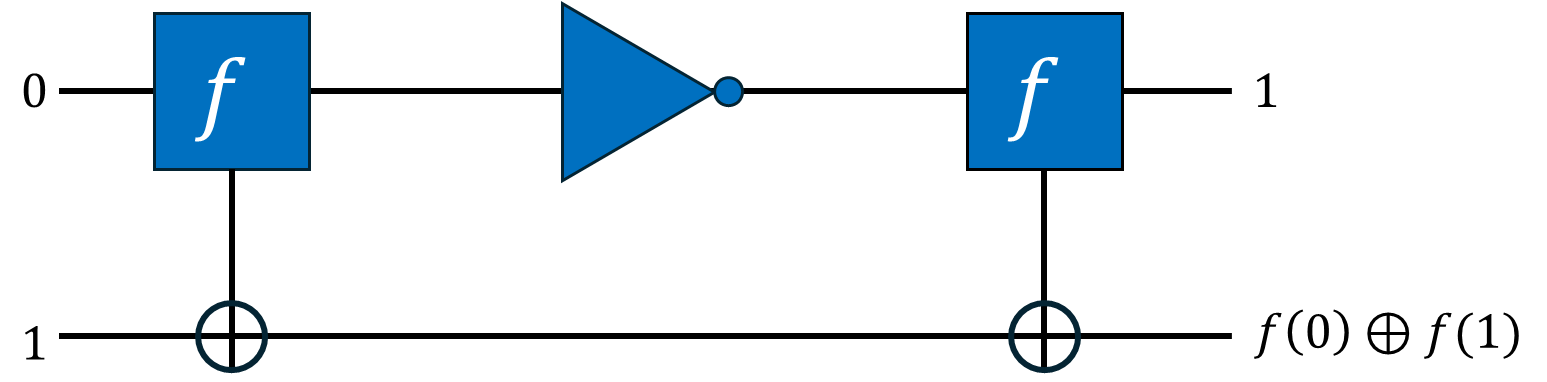
\includegraphics[width=1\linewidth]{Images/Deutsch_classical.png}
    \caption{Classical Deutsch Circuit}
    \label{fig:classical_deutsch}
\end{figure}

The first query XORs the value of $f(0)$ to the second bit. Then, the first bit is flipped to 1, so the second query XORs the value of $f(1)$ to the second bit. At the end, the second bit contains the value of $f(0) \oplus f(1)$, which is the solution to Deutsch's problem.

There is an obvious 2-query quantum algorithm that solves Deutsch's problem just like the circuit shown in Figure~\ref{fig:classical_deutsch}.

\section{The Quantum Solution: Deutsch's Algorithm}

\subsection{Quantum Parallelism}

One uniquely quantum-mechanical effect that we can use for building quantum algorithms is quantum parallelism. Suppose we have a classical algorithm that computes some function $f:\{0,1\}^n \rightarrow \{0,1\}^m$. Then we can build a quantum circuit $U$ (consisting only of Toffoli gates) that maps $\ket{z}\ket{0} \rightarrow \ket{z}\ket{f(z)}$ for every $z \in \{0,1\}^n$. 

Now suppose we apply $U$ to a superposition of all inputs $z$ (which is easy to build using $n$ Hadamard transformations):
\[
U\left(\frac{1}{\sqrt{2^n}} \sum_{z \in \{0,1\}^n} \ket{z}\ket{0}\right) = \frac{1}{\sqrt{2^n}} \sum_{z \in \{0,1\}^n} \ket{z}\ket{f(z)}
\]

We applied $U$ just once, but the final superposition contains $f(z)$ for all $2^n$ input values $z$! However, by itself, this is not very useful and does not give more than classical randomization, since observing the final superposition will give just one uniformly random $\ket{z}\ket{f(z)}$, and all other information will be lost. As we will see below, quantum parallelism needs to be combined with the effects of interference and entanglement in order to achieve something that is better than classical.

\textbf{On a Quantum Computer:} To solve this problem on a quantum computer using Deutsch's Algorithm, we are required to make only one function call. This speedup is possible because of superposition.

Now, when we consider the same question in the context of quantum information, we need to change the question slightly in order for it to fit into the model of quantum information that we are considering. More specifically, we must insist that the action of the device corresponds to a unitary transformation. It is therefore not sufficient to consider the black box to be a one-qubit action, as shown below:

\begin{figure}[ht]
    \centering
    \begin{quantikz}
        \lstick{$\ket{a}$} & \gate{f} & \rstick{$\ket{f(a)}$}
    \end{quantikz}
\end{figure}

For example, if $f = f_3$, then this gate would correspond to the matrix:
\[
\begin{pmatrix}
1 & 1 \\
0 & 0
\end{pmatrix}
\]
which is not unitary.

Instead, for any function $f: \{0,1\} \rightarrow \{0,1\}$, we define a 2-qubit quantum gate $B_f$ as follows:

\begin{figure}[ht]
    \centering
    \begin{quantikz}
        \lstick{$\ket{a}$} & \gate[2]{U_f} & \rstick{$\ket{a}$}\\
        \lstick{$\ket{b}$} &  & \rstick{$\ket{b\oplus f(a)}$}
    \end{quantikz}
    \caption{Oracle}
    \label{fig:deutsch_oracle}
\end{figure}

It can be verified that the corresponding matrix is unitary for any function $f$. For example, if $f = f_4$ from Table~\ref{tab:Deutsch}, then $f(0) = 1$ and $f(1) = 0$, so the corresponding matrix is:
\[
\begin{pmatrix}
0 & 1 & 0 & 0 \\
1 & 0 & 0 & 0 \\
0 & 0 & 1 & 0 \\
0 & 0 & 0 & 1
\end{pmatrix}
\]

For any function $f$, the matrix corresponding to $U_f$ will always be a permutation matrix, meaning that all of the entries are 0 or 1 and every row and every column has exactly one 1 in it. Permutation matrices are always unitary.

In general, if
\[
f: \{0,1\}^n \rightarrow \{0,1\}^m
\]
is any function (for any positive integers $n$ and $m$), the associated quantum transformation $U_f$ is defined by
\[
U_f\ket{x}\ket{y} = \ket{x}\ket{y \oplus f(x)}
\]
where $\oplus$ denotes the bitwise exclusive OR. The associated matrix will always be a permutation matrix, and is therefore unitary. Note that we generally assume the second input to the oracle to be $\ket{0}$, so this simplifies the oracle as follows:
\[
U_f\ket{x}\ket{0} = \ket{x}\ket{0 \oplus f(x)} = \ket{x}\ket{f(x)}
\]

The circuit for Deutsch's Algorithm is shown in Figure~\ref{fig:deutsch}.

\begin{figure}[ht]
    \centering
    \begin{quantikz}
        \lstick{$q_0 = \ket{0}$} & & \gate{H} & \gate[2]{U_f} & \gate{H} & \meter{}\\
        \lstick{$q_1 = \ket{0}$} & \gate{X} & \gate{H} &  & & 
    \end{quantikz}
    \caption{Deutsch's Algorithm}
    \label{fig:deutsch}
\end{figure}

Here the oracle is as shown in Figure~\ref{fig:deutsch_oracle}. The oracle is a black box which takes inputs $\ket{x}$ and $\ket{y}$ and outputs $\ket{x}$ and $\ket{y \oplus f(x)}$. It is a unitary operator (denoted by $U_f$) and implements the function $f$.


\subsection{Idea of the Algorithm}
The primary limitation of the classical algorithm is that we can input either $0$ or $1$ to the reversible classical query—but not both simultaneously. This limitation arises from the classical laws of physics, which prevent us from computing the solution in a single query and instead require two separate queries. 

This classical limitation is overcome in the quantum case. The input to the black-box (or quantum oracle) can be a superposition of $\ket{0}$ and $\ket{1}$, thus allowing simultaneous evaluation of both inputs $0$ and $1$ to the function. Then, through specific quantum manipulations (such as applying Hadamard gates before and after the oracle), and upon measurement, we can obtain a result that clearly distinguishes the two classical outcomes—either $0$ or $1$—enabling us to determine whether the function $f$ is constant or balanced. 

This capability arises from the power of quantum superposition applied to the states $\ket{0}$ and $\ket{1}$. It is this core feature of quantum mechanics that enables Deutsch's algorithm to identify the nature of the function $f$ in a single query.

\subsection{Algorithm}
The details are given in the algorithm~\ref{algo:deutsch}.
\begin{algorithm}
    \caption{Deutsch Algorithm}
    \begin{algorithmic}[1]
    \State \textbf{Input:} A black box $U_f$ which performs the transformation $\ket{x}\ket{y} \rightarrow \ket{x}\ket{y \oplus f(x)}$, for $x \in \{0,1\}$ and $f(x) \in \{0,1\}$. It is promised that $f(x)$ is either constant for all values of $x$, or balanced, i.e., equal to $1$ for exactly half of all the possible $x$, and $0$ for the other half.
    \State \textbf{Output:} $0$ if $f$ is constant and $1$ if $f$ is balanced.
    \State \textbf{Runtime:} One evaluation of $U_f$. Always succeeds.
    \State \textbf{Initialize:} $\ket{00}$
    \State Apply NOT gate to the last qubit:
    \[
    \rightarrow \ket{01}
    \]
    \State Create superposition using Hadamard gates:
    \[
    \rightarrow \left(\frac{\ket{0}+\ket{1}}{\sqrt{2}}\right) \left(\frac{\ket{0} - \ket{1}}{\sqrt{2}}\right)
    \]
    \State Calculate function $f$ using $U_f$:
    \[
    \rightarrow  (-1)^{f(0)}\frac{(\ket{0}+(-1)^{f(0)\oplus f(1)}\ket{1})}{\sqrt{2}} \left(\frac{\ket{0} - \ket{1}}{\sqrt{2}}\right)
    \]
    \State Perform Hadamard transform:
    \[
    \rightarrow (-1)^{f(0)} \ket{f(0)\oplus f(1)} \left(\frac{\ket{0} - \ket{1}}{\sqrt{2}}\right)
    \]
    \State Measure the first qubit to obtain the final output $\ket{f(0)\oplus f(1)}$
    \State If $0$ \textbf{return} constant; if $1$ \textbf{return} balanced.
    \end{algorithmic}
    \label{algo:deutsch}
\end{algorithm}
\textbf{Claim: }If upon measurement of the first qubit, the result is $\ket{0}$, then the function is constant; otherwise, the function is balanced.\\
\textbf{Analysis: }Initially, both qubits are in the state $q_0 = \ket{0}$ and $q_1 = \ket{0}$. After passing through Hadamard and Pauli-X gates:

\begin{itemize}
    \item The first qubit $q_0$ becomes $\ket{+} = \frac{1}{\sqrt{2}}(\ket{0} + \ket{1})$ after a Hadamard gate.
    \item The second qubit $q_1$ is passed through an $X$ gate, becoming $\ket{1}$, and then through a Hadamard gate, becoming $\ket{-} = \frac{\ket{0} - \ket{1}}{\sqrt{2}}$.
\end{itemize}

Thus, the state at the input to the oracle is:
\[
\ket{+} \otimes \ket{-}
\]

The action of the oracle is defined as:
\[
U_f \ket{x} \ket{y} = \ket{x} \ket{y \oplus f(x)}
\]

Apply $U_f$ to the input state:
\begin{align*}
U_f \ket{+} \ket{-} &= U_f \left( \frac{1}{\sqrt{2}}(\ket{0} + \ket{1}) \otimes \frac{1}{\sqrt{2}}(\ket{0} - \ket{1}) \right) \\
&= \frac{1}{2} \left( \ket{0}(\ket{0 \oplus f(0)} - \ket{1 \oplus f(0)}) + \ket{1}(\ket{0 \oplus f(1)} - \ket{1 \oplus f(1)}) \right)
\end{align*}

Now, using the identity:
\[
\ket{0 \oplus a} - \ket{1 \oplus a} = (-1)^a (\ket{0} - \ket{1})
\]
we can simplify:
\begin{align*}
&= \frac{1}{2} \left[ (-1)^{f(0)}\ket{0} + (-1)^{f(1)}\ket{1} \right] \otimes (\ket{0} - \ket{1}) \\
&= \left( \frac{1}{\sqrt{2}} \left[ (-1)^{f(0)} \ket{0} + (-1)^{f(1)} \ket{1} \right] \right) \otimes \left( \frac{1}{\sqrt{2}} (\ket{0} - \ket{1}) \right) \\
&= \left( \frac{1}{\sqrt{2}} \left[ (-1)^{f(0)} \ket{0} + (-1)^{f(1)} \ket{1} \right] \right) \otimes \ket{-}
\end{align*}

Factoring out $(-1)^{f(0)}$:
\[
= (-1)^{f(0)} \left( \frac{1}{\sqrt{2}} \left[ \ket{0} + (-1)^{f(0) \oplus f(1)} \ket{1} \right] \right) \otimes \ket{-}
\]

Note that $(-1)^{f(0)}$ is not a global phase unless the first qubit is in a computational basis state. Here, since the first qubit is in a superposition, the relative phase matters and carries information.

Now, apply the Hadamard gate on the first qubit:
\begin{align*}
(H \otimes I) & \left[ \left( \frac{1}{\sqrt{2}} \left( \ket{0} + (-1)^{f(0) \oplus f(1)} \ket{1} \right) \right) \otimes (-1)^{f(0)} \ket{-} \right] \\
&= \ket{f(0) \oplus f(1)} \otimes (-1)^{f(0)} \ket{-}
\end{align*}

Here, we have used the identity:
\[
H \left( \frac{1}{\sqrt{2}} (\ket{0} + (-1)^a \ket{1}) \right) = \ket{a}
\quad \text{for } a \in \{0,1\}
\]

Therefore, upon measurement of the first qubit, we obtain the value $f(0) \oplus f(1)$ with certainty:
\begin{itemize}
    \item If $f$ is constant, then $f(0) = f(1)$, so $f(0) \oplus f(1) = 0$ and we observe $\ket{0}$.
    \item If $f$ is balanced, then $f(0) \neq f(1)$, so $f(0) \oplus f(1) = 1$ and we observe $\ket{1}$.
\end{itemize}
This completes the analysis of Deutsch’s algorithm, which determines whether the function $f$ is constant or balanced using only a single query to the oracle.

\section*{Analysis of Deutsch's Algorithm}

For further explanation, consider the following cases:

\begin{enumerate}
    \item \textbf{Case 1: Function is Constant with $f(0)=f(1)=0$} \\
    If the function is constant, then $f(0) = f(1)$. Let $f(0) = f(1) = 0$, then the output of the oracle will be:
    \[
        \frac{1}{2}\left(\ket{0}\ket{0} - \ket{0}\ket{1} + \ket{1}\ket{0} - \ket{1}\ket{1}\right)
    \]
    This expression can be factorized into a tensor product of two states:
    \[
        = \frac{\ket{0} + \ket{1}}{\sqrt{2}} \otimes \frac{\ket{0} - \ket{1}}{\sqrt{2}} = \ket{+} \otimes \ket{-}
    \]
    Applying $(H \otimes I)$ gives:
    \[
        (H \otimes I)(\ket{+} \otimes \ket{-}) = \ket{0} \otimes \ket{-}
    \]
    Therefore, after applying Hadamard to the first qubit, the state becomes $\ket{0} \otimes \ket{-}$. Measuring the first qubit yields outcome $0$ with probability $1$.

    \item \textbf{Case 2: Function is Constant with $f(0)=f(1)=1$} \\
    Again, since the function is constant, $f(0) = f(1)$. Let $f(0) = f(1) = 1$. The output of the oracle is:
    \[
        \frac{1}{2}\left(\ket{0}\ket{1} - \ket{0}\ket{0} + \ket{1}\ket{1} - \ket{1}\ket{0}\right)
    \]
    Factorizing:
    \[
        = \frac{\ket{0} + \ket{1}}{\sqrt{2}} \otimes \left(-\frac{\ket{0} - \ket{1}}{\sqrt{2}}\right) = \ket{+} \otimes -\ket{-}
    \]
    Applying $(H \otimes I)$:
    \[
        (H \otimes I)(\ket{+} \otimes -\ket{-}) = \ket{0} \otimes -\ket{-}
    \]
    Measuring the first qubit gives outcome $0$ with probability $1$.

    \item \textbf{Case 3: Function is Balanced with $f(0)=0$ and $f(1)=1$} \\
    If the function is balanced, then $f(0) \neq f(1)$. Let $f(0) = 0$, $f(1) = 1$. The oracle output is:
    \[
        \frac{1}{2}\left(\ket{0}\ket{0} - \ket{0}\ket{1} + \ket{1}\ket{1} - \ket{1}\ket{0}\right)
    \]
    Factorizing:
    \[
        = \frac{\ket{0} - \ket{1}}{\sqrt{2}} \otimes \frac{\ket{0} - \ket{1}}{\sqrt{2}} = \ket{-} \otimes \ket{-}
    \]
    Applying $(H \otimes I)$:
    \[
        (H \otimes I)(\ket{-} \otimes \ket{-}) = \ket{1} \otimes \ket{-}
    \]
    Measuring the first qubit yields outcome $1$ with probability $1$.

    \item \textbf{Case 4: Function is Balanced with $f(0)=1$ and $f(1)=0$} \\
    Again, $f(0) \neq f(1)$. Let $f(0) = 1$, $f(1) = 0$. The oracle output is:
    \[
        \frac{1}{2}\left(\ket{0}\ket{1} - \ket{0}\ket{0} + \ket{1}\ket{0} - \ket{1}\ket{1}\right)
    \]
    Factorizing:
    \[
        = \frac{\ket{0} - \ket{1}}{\sqrt{2}} \otimes \left(-\frac{\ket{0} - \ket{1}}{\sqrt{2}}\right) = \ket{-} \otimes -\ket{-}
    \]
    Applying $(H \otimes I)$:
    \[
        (H \otimes I)(\ket{-} \otimes -\ket{-}) = \ket{1} \otimes -\ket{-}
    \]
    Measuring the first qubit yields outcome $1$ with probability $1$.
\end{enumerate}

\vspace{0.5cm}
It is important to note the role of Hadamard gates in this algorithm:

\begin{itemize}
    \item The first Hadamard gate applied to the input $\ket{0}$ prepares the superposition $\ket{+} = \frac{\ket{0} + \ket{1}}{\sqrt{2}}$.
    \item The Hadamard on the second qubit, initialized in state $\ket{1}$, produces $\ket{-} = \frac{\ket{0} - \ket{1}}{\sqrt{2}}$.
\end{itemize}

This $\ket{-}$ state is crucial because the oracle acts as:
\[
    \ket{x}\ket{-} \rightarrow (-1)^{f(x)}\ket{x}\ket{-}
\]
Thus, the oracle applies a phase $(-1)^{f(x)}$ to each basis state $\ket{x}$, and the overall result is:
\[
    \frac{1}{\sqrt{2}} \left( (-1)^{f(0)}\ket{0} + (-1)^{f(1)}\ket{1} \right) \otimes \ket{-}
\]

After the second Hadamard gate is applied to the first qubit, the output becomes:
\[
    H\left( \frac{(-1)^{f(0)}\ket{0} + (-1)^{f(1)}\ket{1}}{\sqrt{2}} \right) = \ket{f(0) \oplus f(1)}
\]
Therefore, measurement of the first qubit gives:

\begin{itemize}
    \item $\ket{0}$ if the function is constant ($f(0) \oplus f(1) = 0$)
    \item $\ket{1}$ if the function is balanced ($f(0) \oplus f(1) = 1$)
\end{itemize}

This allows us to determine whether the function is constant or balanced using only \textbf{one} query to the oracle. This is a quantum speedup over the classical algorithm, which requires \textbf{two} function evaluations to determine the same information.

\paragraph{Important Observation:} This algorithm does \textbf{not} reveal the individual values of $f(0)$ or $f(1)$. It only reveals the XOR of the two: $f(0) \oplus f(1)$. Running this algorithm gives no information about the values of $f(0)$ or $f(1)$ themselves.


\subsection{Example}
\begin{example}
    \textbf{(One-out-of-four search)} Let $f:\{0,1\}^2 \rightarrow \{0,1\}$ have the special property that it attains the value 1 at exactly one of the four points in its domain. There are four such possible functions, each corresponding to a unique input where the output is 1. The truth tables for these functions are shown in table~\ref{tab:deutsch_example}.

    \begin{table}[ht]
    \centering
     \begin{subtable}[b]{0.45\linewidth}
        \centering
          \begin{tabular}{|c|c|c|}
            \hline
             Function & Input & Output \\
            \hline
              $f_{00}$& 00 & 1 \\
              & 01 & 0 \\
              & 10 & 0 \\
              & 11 & 0 \\
             \hline
           \end{tabular}
           \caption{$f_{00}$}
        \end{subtable}%
     \begin{subtable}[b]{0.45\linewidth}
            \centering
            \begin{tabular}{|c|c|c|}
                \hline
                Function & Input & Output \\
                \hline
                $f_{01}$& 00 & 0 \\
                & 01 & 1 \\
                & 10 & 0 \\
                & 11 & 0 \\
                \hline
            \end{tabular}
            \caption{$f_{01}$}
        \end{subtable}
        \begin{subtable}[b]{0.45\linewidth}
            \centering
            \begin{tabular}{|c|c|c|}
                \hline
                Function & Input & Output \\
                \hline
                $f_{10}$& 00 & 0 \\
                & 01 & 0 \\
                & 10 & 1 \\
                & 11 & 0 \\
                \hline
            \end{tabular}
            \caption{$f_{10}$}
        \end{subtable}
        \begin{subtable}[b]{0.45\linewidth}
            \centering
            \begin{tabular}{|c|c|c|}
                \hline
                Function & Input & Output \\
                \hline
                $f_{11}$& 00 & 0 \\
                & 01 & 0 \\
                & 10 & 0 \\
                & 11 & 1 \\
                \hline
            \end{tabular}
            \caption{$f_{11}$}
        \end{subtable}
        \caption{Possible functions with a unique solution}
        \label{tab:deutsch_example}
    \end{table}

    The goal is to determine which one of these four functions is implemented by a given black-box. In other words, you're given black-box access to a function $f$ with the promise that $f$ is one of the above functions. Access to the function is restricted to evaluations via the transformation $B_f$. Each evaluation of $B_f$ on a chosen input (classical or quantum) is considered a query.

    You're promised that $f$ outputs 1 at exactly one input and 0 at all others, but you're not told which input this is. Your task is to identify the correct function, which can be thought of as solving a simple search problem.

Classically, three queries are sufficient to solve the problem. You can query the function in the first three positions and check whether any of them evaluates to 1. If none of them do, then by process of elimination, you can deduce that the 1 must be at the fourth position.

In the quantum case, however, one query is sufficient to solve the problem. Here, the oracle performs operations implementing the function that maps two bits to one bit as
\[
U_f\ket{x}\ket{y}\ket{z} = \ket{x}\ket{y}\ket{z \oplus f(x,y)},
\]
where there are two qubits for the input and a third qubit for the output. In the computational basis, the value of $f(x, y)$ is XORed onto the third qubit. This description holds for basis states, but it extends linearly to superpositions.

As in Deutsch’s algorithm, we set the target qubit to the state $\ket{-}$ to enable phase kickback and prepare the input qubits in a uniform superposition.

\begin{figure}[H]
    \centering
    \begin{quantikz}
        \lstick{$\ket{0}$} & & \gate{H} & \gate[3]{U_f} & \gate{H}\gategroup[2,steps=4,style={dashed,rounded corners, , inner xsep=2pt},background,label style={label position=above, anchor=south, yshift=-0.2cm}]{{\sc $U$}} & \gate{Z}   & \ctrl{1} & \gate{H} & \meter{} \\
        \lstick{$\ket{0}$} & & \gate{H} &                            & \gate{H} & \gate{Z} & \control{} & \gate{H} & \meter{} \\
        \lstick{$\ket{0}$} & \gate{X} & \gate{H} &                  &          &          &            &          &
    \end{quantikz}
    \caption{Quantum Circuit}
    \label{fig:deutsch_example}
\end{figure}

Consider the circuit in Figure~\ref{fig:deutsch_example}. After the Hadamard transforms and before the query, the state becomes:
\[
\left(\frac{1}{2}\ket{00} + \frac{1}{2}\ket{01} + \frac{1}{2}\ket{10} + \frac{1}{2}\ket{11}\right) \otimes \left(\frac{1}{\sqrt{2}}\ket{0} - \frac{1}{\sqrt{2}}\ket{1}\right).
\]

After the oracle $U_f$ is applied, the state becomes:
\[
\left(\frac{1}{2}(-1)^{f(00)}\ket{00} + \frac{1}{2}(-1)^{f(01)}\ket{01} + \frac{1}{2}(-1)^{f(10)}\ket{10} + \frac{1}{2}(-1)^{f(11)}\ket{11}\right) \otimes \left(\frac{1}{\sqrt{2}}\ket{0} - \frac{1}{\sqrt{2}}\ket{1}\right).
\]

This works because of the \textbf{\textit{phase kickback effect}}, just as in Deutsch’s algorithm.

Now, depending on where the function outputs 1, we are left with four possibilities for the first two qubits:
\begin{align*}
f = f_{00} &\implies \ket{\phi_{00}} = -\frac{1}{2}\ket{00} + \frac{1}{2}\ket{01} + \frac{1}{2}\ket{10} + \frac{1}{2}\ket{11}, \\
f = f_{01} &\implies \ket{\phi_{01}} = \frac{1}{2}\ket{00} - \frac{1}{2}\ket{01} + \frac{1}{2}\ket{10} + \frac{1}{2}\ket{11}, \\
f = f_{10} &\implies \ket{\phi_{10}} = \frac{1}{2}\ket{00} + \frac{1}{2}\ket{01} - \frac{1}{2}\ket{10} + \frac{1}{2}\ket{11}, \\
f = f_{11} &\implies \ket{\phi_{11}} = \frac{1}{2}\ket{00} + \frac{1}{2}\ket{01} + \frac{1}{2}\ket{10} - \frac{1}{2}\ket{11}.
\end{align*}

Note that these four states form an orthonormal set:
\[
\braket{\phi_{ab} | \phi_{cd}} = 
\begin{cases}
1 & \text{if } a = c \text{ and } b = d, \\
0 & \text{otherwise}.
\end{cases}
\]

Whenever you have an orthonormal set like this, it is always possible to construct a quantum circuit that exactly distinguishes these states. In fact, the corresponding unitary transformation is easy to obtain: let the vectors form the columns of a matrix and then take the conjugate transpose. The matrix $U$ that performs this transformation is:
\[
U = \begin{pmatrix}
-\frac{1}{2} & \frac{1}{2} & \frac{1}{2} & \frac{1}{2} \\
\frac{1}{2} & -\frac{1}{2} & \frac{1}{2} & \frac{1}{2} \\
\frac{1}{2} & \frac{1}{2} & -\frac{1}{2} & \frac{1}{2} \\
\frac{1}{2} & \frac{1}{2} & \frac{1}{2} & -\frac{1}{2}
\end{pmatrix}=\frac{1}{2}\begin{pmatrix}
    -1 & 1 & 1 & 1 \\
    1 & -1 & 1 & 1 \\
    1 & 1 & -1 & 1 \\
    1 & 1 & 1 & -1
\end{pmatrix}.
\]

You can verify that $U\ket{\phi_{ab}} = \ket{ab}$ for all $a, b \in \{0, 1\}$.

To implement this unitary, we use a series of gates, as shown in Figure~\ref{fig:deutsch_example}. The transformation includes the phase flip (Pauli-Z) gate:
\[
Z = \begin{pmatrix}
1 & 0 \\
0 & -1
\end{pmatrix},
\]
as well as a controlled-Z (CZ) gate, where the first qubit is the control and the second is the target.
\end{example}

One can try to implement all the four functions in oracles and simulate the results on a quantum computer.

\section{Implementation using Qiskit}
\subsection{Background}

To run Deutsch's algorithm, we require an oracle that implements a function—either constant or balanced—and a circuit to evaluate it. Here, we demonstrate how to construct such oracles and use gates from the Qiskit Circuit Library to build Deutsch's circuit. The \texttt{Sampler} primitive in Qiskit Runtime allows for seamless execution of the circuit.

\vspace{0.5em}
\noindent\textbf{Note:} The estimated runtime is approximately 4 seconds; actual runtimes may vary depending on backend load and network conditions.

\subsection{Requirements}

Before starting this tutorial, ensure that the following dependencies are installed:
\begin{itemize}
    \item Qiskit SDK 1.0 or later with visualization support: \texttt{pip install 'qiskit[visualization]'}
    \item Qiskit Runtime 0.22 or later: \texttt{pip install qiskit-ibm-runtime}
\end{itemize}

\subsection{Setup}

We begin by importing the essential Python modules and Qiskit components required for this demonstration.

\begin{lstlisting}[language=Python, caption={Importing Required Modules}]
#Built-in modules
import math

#imports from Qiskit
from qiskit import QuantumCircuit, QuantumRegister, ClassicalRegister
from qiskit.visualization import plot_distribution, plot_histogram
from qiskit_aer import AerSimulator
from qiskit.transpiler.preset_passmanagers import generate_preset_pass_manager


#Imports from Qiskit Primitives
from qiskit_ibm_runtime import SamplerV2 as Sampler

#Imports from Qiskit Runtime
from qiskit_ibm_runtime import QiskitRuntimeService
\end{lstlisting}

If you wish to run the circuit on real quantum hardware rather than a simulator, the following code will help you choose the least busy operational backend.

\begin{lstlisting}[language=Python, caption={Connecting to Quantum Hardware}]
# To run on hardware, select the backend with the fewest number of jobs in the queue
# backend = AerSimulator()  # Use AerSimulator for local simulation

# To run on IBM Quantum hardware, uncomment the following lines
service = QiskitRuntimeService(channel="ibm_quantum")
backend = service.least_busy(operational=True, simulator=False)
backend.name
\end{lstlisting}

This outputs the name of one of IBM's quantum computers (e.g., \texttt{`ibm\_brisbane'}).

\begin{enumerate}
    \item \textbf{Step 1: Map classical inputs to a quantum problem}: \\
    There are four possibilities for the oracles in Deutsch's algorithm, where the oracle implements a function $f: \{0,1\} \rightarrow \{0,1\}$. The function can be either constant ($f_1$ or $f_2$) or balanced ($f_3$ or $f_4$), as given in Table~\ref{tab:Deutsch}. The code for creating the Deutsch circuit is as follows:

\begin{lstlisting}[language=Python]
def deutsch_circuit(value):
    # Create a Quantum Circuit
    qubits = QuantumRegister(2, name="q")
    cbits = ClassicalRegister(1, name="c")
    circuit = QuantumCircuit(qubits, cbits)

    q0, q1 = qubits
    circuit.h(q0)
    circuit.x(q1)
    circuit.h(q1)

    circuit.barrier()
    if value == 1:
        circuit.id(q0)
        circuit.id(q1)
    elif value == 2:
        circuit.id(q0)
        circuit.x(q1)
    elif value == 3:
        circuit.cx(q0, q1)
    elif value == 4:
        circuit.cx(q0, q1)
        circuit.x(q1)

    circuit.barrier()
    circuit.h(q0)

    circuit.measure(q0, 0)

    return circuit
\end{lstlisting}

    To create one of the circuits, use the following code:

\begin{lstlisting}[language=Python]
qc_4 = deutsch_circuit(value=4)
qc_4.draw("mpl")
\end{lstlisting}

    All the circuits, along with their corresponding oracles implementing the four functions, are shown in the figure~\ref{fig:deutsch_circuit}:

    \begin{figure}[ht]
        \centering
        \begin{subfigure}[b]{0.45\linewidth}
            \centering
            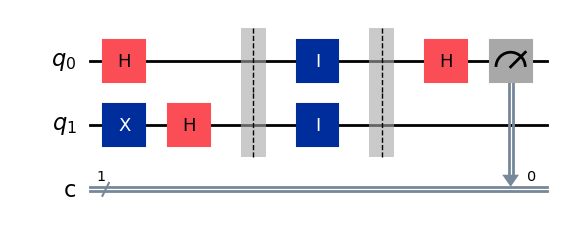
\includegraphics[width=1\linewidth]{Images/deutsch_f1.png}
            \caption{$f = f_1$}
            \label{fig:deutsch_f1}
        \end{subfigure}
        \hfill
        \begin{subfigure}[b]{0.45\linewidth}
            \centering
            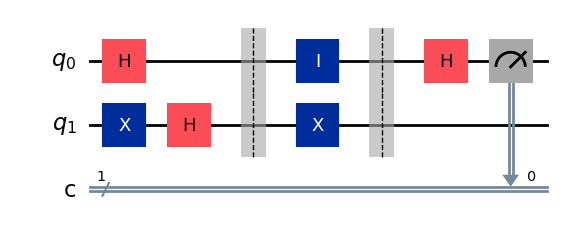
\includegraphics[width=1\linewidth]{Images/deutsch_f2.png}
            \caption{$f = f_2$}
            \label{fig:deutsch_f2}
        \end{subfigure}
        \vspace{0.5cm}
        \begin{subfigure}[b]{0.45\linewidth}
            \centering
            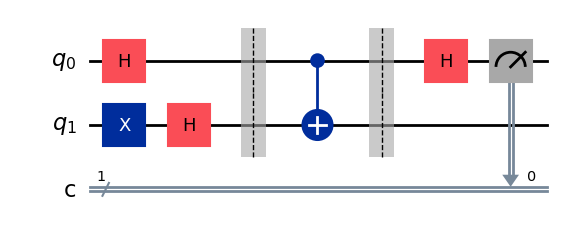
\includegraphics[width=1\linewidth]{Images/deutsch_f3.png}
            \caption{$f = f_3$}
            \label{fig:deutsch_f3}
        \end{subfigure}
        \hfill
        \begin{subfigure}[b]{0.45\linewidth}
            \centering
            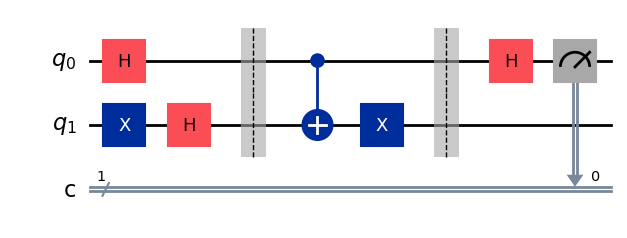
\includegraphics[width=1\linewidth]{Images/deutsch_f4.png}
            \caption{$f = f_4$}
            \label{fig:deutsch_f4}
        \end{subfigure}
        \caption{Deutsch circuit implementations for all possible functions, along with their corresponding oracles}
        \label{fig:deutsch_circuit}
    \end{figure}

    Note that each oracle (implemented between the two barriers) realizes one of the required functions. Thus, the figure above illustrates the complete Deutsch circuit for each of the four function cases.

    \item \textbf{Step 2: Optimize the circuit for quantum execution}
    
    To optimize the circuit for the chosen backend, you can use the Qiskit transpiler with a high optimization level:

\begin{lstlisting}[language=Python]
target=backend.target
pm = generate_preset_pass_manager(backend=backend, optimization_level=3)

circuit_isa_4=pm.run(qc_4)
circuit_isa_4.draw(output="mpl")
\end{lstlisting}
The circuits after optimization are as shown in figure~\ref{fig:opt_deutsch_circuit}.
   \begin{figure}[ht]
    \centering
    \begin{subfigure}[b]{0.6\linewidth}
        \centering
        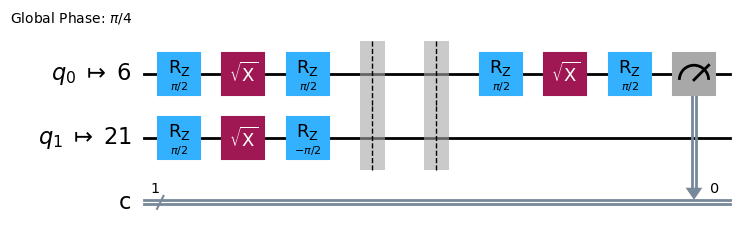
\includegraphics[width=1\linewidth]{Images/opt_deutsch_f1.png}
        \caption{$f = f_1$}
        \label{fig:opt_deutsch_f1}
    \end{subfigure}
    \hfill
    \begin{subfigure}[b]{0.6\linewidth}
        \centering
        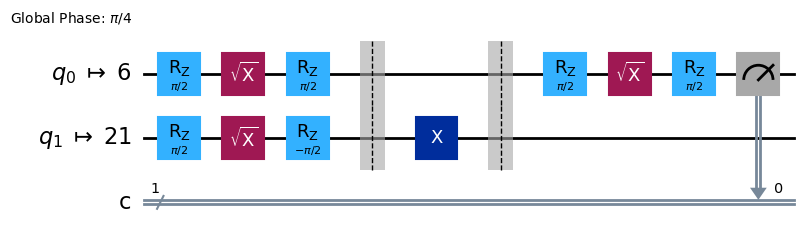
\includegraphics[width=1\linewidth]{Images/opt_deutsch_f2.png}
        \caption{$f = f_2$}
        \label{fig:opt_deutsch_f2}
    \end{subfigure}
    \vspace{0.5cm}
    \begin{subfigure}[b]{0.6\linewidth}
        \centering
        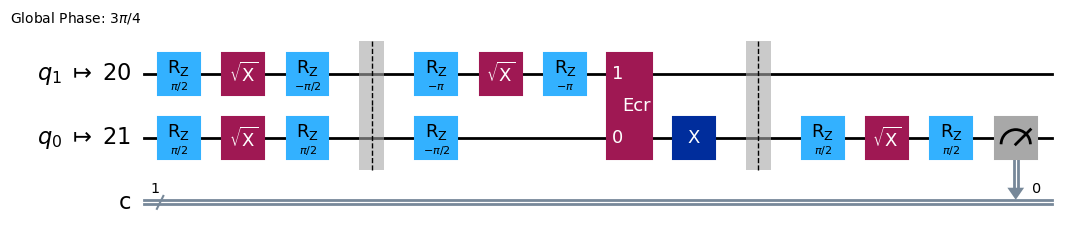
\includegraphics[width=1\linewidth]{Images/opt_deutsch_f3.png}
        \caption{$f = f_3$}
        \label{fig:opt_deutsch_f3}
    \end{subfigure}
    \hfill
    \begin{subfigure}[b]{0.6\textwidth}
        \centering
        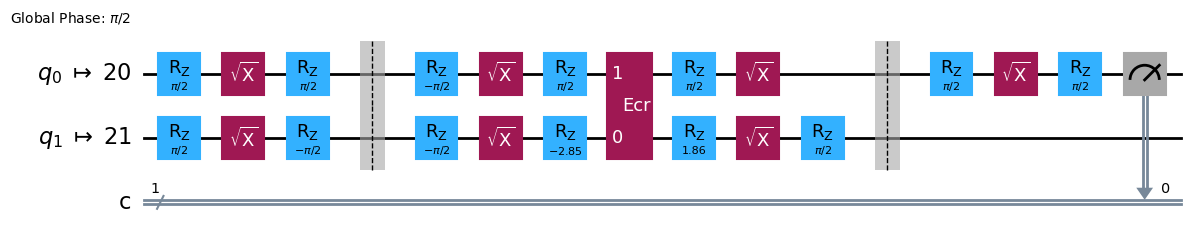
\includegraphics[width=1\linewidth]{Images/opt_deutsch_f4.png}
        \caption{$f = f_4$}
        \label{fig:opt_deutsch_f4}
    \end{subfigure}    
    \caption{Corresponding optimized Deutsch circuits for different oracle functions}
    \label{fig:opt_deutsch_circuit}
\end{figure}
    \item \textbf{Step 3: Execute using Qiskit Primitives} \\
    We now run the circuit and sample the measurements on the first qubit. For this execution, we use the \texttt{Sampler} runtime primitive.
    
\begin{lstlisting}[language=Python]
sampler=Sampler(mode=backend)
sampler.options.default_shots=10_000
result_4 = sampler.run([circuit_isa_4]).result()
dist_4 = result_4[0].data.c.get_counts()
\end{lstlisting}
The output of the above code will be the distribution of the measurements on the first qubit. Similar code can be written for all four possible functions.

    \item \textbf{Step 4: Post-Process Results} \\
    Now we plot a histogram of the measurements on the first qubit in classical format.
    
\begin{lstlisting}[language=Python]
from qiskit.visualization import plot_histogram
plot_histogram(dist_1)
\end{lstlisting}
    The output of the above code will be the histogram showing the distribution of the measurements on the first qubit. The histograms are as shown in figure~\ref{fig:deutsch_results}. Similar code can be used for all four oracle implementations.


    The following output is produced upon executing the above code on the \texttt{ibm\_brisbane} quantum backend, as shown in Figure~\ref{fig:deutsch_results}. The histogram plots were generated using 10{,}000 shots. As observed, the results align closely with theoretical expectations. Minor deviations are present, which are attributed to inherent noise and the probabilistic nature of quantum measurements.

\begin{figure}[ht]
    \centering
    \begin{subfigure}[b]{0.45\linewidth}
    \centering
    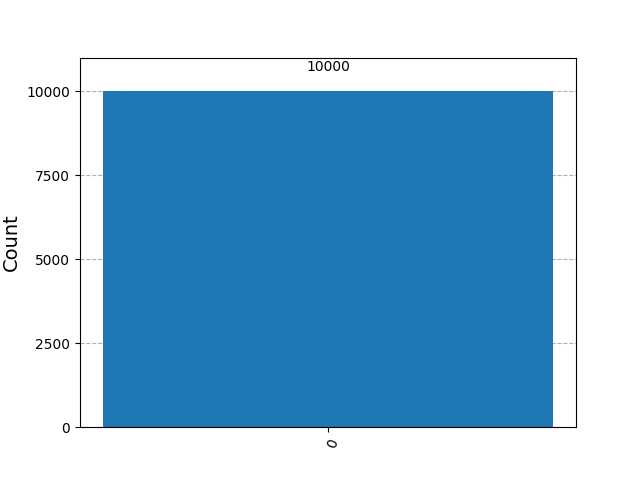
\includegraphics[width=1\linewidth]{Images/deutsch_result_f1.png}
    \caption{$f = f_1 \implies \text{constant}$}
    \label{fig:deutsch_result_f1}
    \end{subfigure}
    \hfill
    \begin{subfigure}[b]{0.45\linewidth}
    \centering
    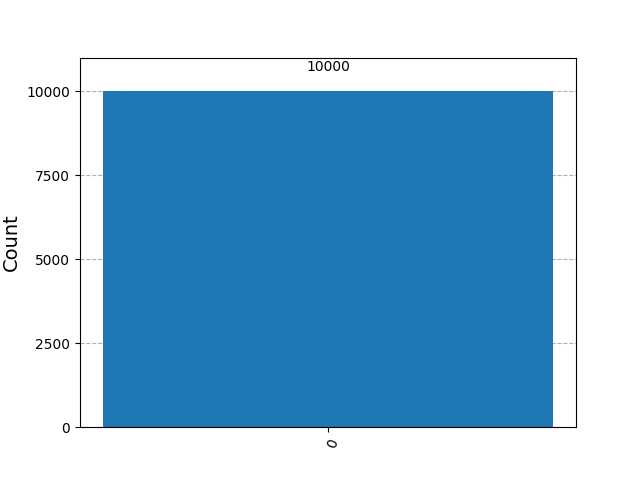
\includegraphics[width=1\linewidth]{Images/deutsch_result_f2.png}
    \caption{$f = f_2 \implies \text{constant}$}
    \label{fig:deutsch_result_f2}
    \end{subfigure}
    \vspace{0.5cm}
    \begin{subfigure}[b]{0.45\linewidth}
    \centering
    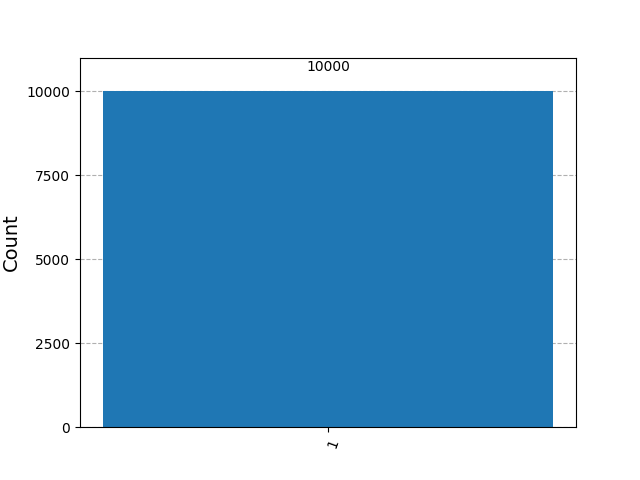
\includegraphics[width=1\linewidth]{Images/deutsch_result_f3.png}
    \caption{$f = f_3 \implies \text{balanced}$}
    \label{fig:deutsch_result_f3}
    \end{subfigure}
    \hfill
    \begin{subfigure}[b]{0.45\linewidth}
    \centering
    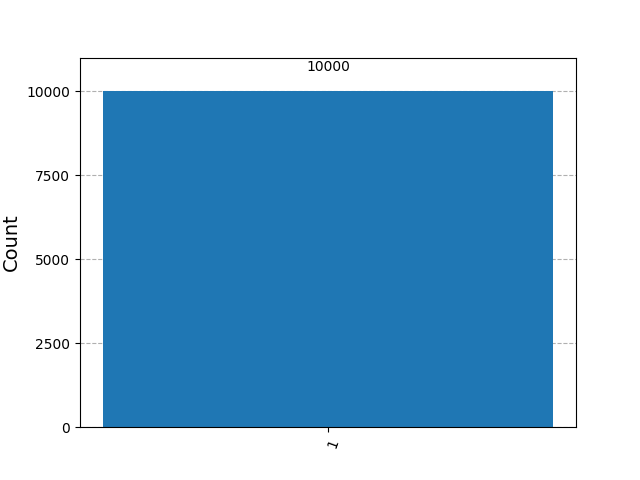
\includegraphics[width=1\linewidth]{Images/deutsch_result_f4.png}
    \caption{$f = f_4 \implies \text{balanced}$}
    \label{fig:deutsch_result_f4}
    \end{subfigure}    
    \caption{Measurement results for all four oracle functions}
    \label{fig:deutsch_results}
\end{figure}

In Figure~\ref{fig:deutsch_result_f1}, the result of measuring the first qubit is $0$ in $9943$ out of $10{,}000$ shots, with the remaining $57$ shots yielding $1$. This strongly indicates that the function implemented inside the oracle was constant, which aligns with our knowledge that $f = f_1$ is indeed a constant function.
\end{enumerate}

Thus, based on the maximum key element from the histogram plot we decide whether the function is constant (if maximum key element is `0') or balanced (if maximum key element is `1'). This can be done as shown in the following code:
\begin{lstlisting}[language=Python]
max_key = max(dist_4, key=dist_4.get)
if max_key == '0':
    print("The function is constant.")
else:
    print("The function is balanced.")
\end{lstlisting}
Similar interpretations can be made for the other functions:
\begin{itemize}
    \item For $f = f_2$, we again observe a dominant outcome of $0$, confirming it as constant.
    \item For $f = f_3$ and $f = f_4$, the dominant measurement outcome is $1$, correctly identifying these as balanced functions.
\end{itemize}

This demonstrates that the Deutsch algorithm enables us to distinguish between constant and balanced functions with just a single quantum query. However, it does not identify the specific function (e.g., $f_1$ vs.\ $f_2$) among the set of possible constant or balanced functions. The results are consistent with theoretical predictions and highlight the correctness of the implemented circuits.

It is important to note that due to noise and hardware imperfections in current quantum devices, the output might slightly vary across different runs. Nonetheless, the results here are a strong validation of the Deutsch algorithm in a real quantum setting.

\begin{remark}
    It is important to note that in this example, we have manually implemented the oracle using basic gates and therefore already know the function it computes. This introduces a caveat in the context of the quantum query model. Ideally, in the query model, the oracle is provided as a black-box function, and the objective is to extract information about it with the minimum number of queries. However, in this demonstration—as well as in the implementations that follow—we construct the oracle ourselves, allowing us to know in advance what the oracle does. We then use the algorithm to verify that it extracts the correct information. From next chapter onwards we will implement the oracle as a black box circuit in the actual algorithm circuit. Also, the optimized circuits and results might vary depending on the system since it is a stochastic process.
\end{remark}



\chapterreferences
